\documentclass[a4paper, 12pt]{article}

\usepackage[utf8]{inputenc}
\usepackage{indentfirst}
\usepackage{amsmath}
\usepackage{bm}
\usepackage{esvect}
\usepackage{graphicx}
\usepackage{hyperref}

\newcommand{\veca}{\[ \vv{a} \]}
\setlength{\parindent}{1cm}
\DeclareMathOperator{\MyFunction}{Fun}


\title{Tutorial}
\author{Gustave Li}
\date{July 2021}


\begin{document}

\maketitle

\section{Change text sizes} \label{sec: text size}

I want to try out different font sizes in this paragraph, this is {\scriptsize smaller than} the original text, this one is {\Large larger}, this one is {\huge even larger}.

\section{Font styles}

\setlength{\parindent}{1cm} 
\noindent This is a normal paragraph.

\noindent \textbf{This is a paragraph with bold texts}

\noindent \textit{This is a paragraph with italics texts}

\noindent \underline{This is a paragraph with underlined texts}

\section{Text emphasis}
Text emphasis in {\LaTeX} is \emph{context driven}, \textbf{which means that the font choice for emphasis text is based on the \emph{current font}}.

\section{Font families}
The default font for {\LaTeX} is Roman, but we can change to \textsf{the sans serif font}.

When typing codes, we may choose typewriter font:
\begin{center}
    \texttt{print('Hello world!')}
    
    \texttt{a = 2}
\end{center}

\section{The tabular environment}
\begin{center}
    \begin{tabular}{|c|c|c|}
    \hline
    text & text & text \\
    \hline
    1    &    2 & 3 \\
    4 & 5 & 6 \\
    \hline
    \end{tabular}
\end{center}


\section{The math environment}
You can enter math formulae in math mode
\[
F = m \times a
\]
\subsection{Display style math}
The formulae are independent from the texts in this style, they are centered separately.

To align several formulae:
\begin{align*}
    f(x) & = a_2 x^2 + a_1 x + a_0 \\
         & = x^2 + 4x -5
\end{align*}

The formulae can also be numbered:
\begin{align}
    f(x) & = a_2 x^2 + a_1 x + a_0 \\
         & = x^2 + 4x -5
\end{align}

Or can only number the last formula:
\begin{align}
    f(x) & = a_2 x^2 + a_1 x + a_0 \nonumber \\
         & = x^2 + 4x -5 
\end{align}

\subsection{Inline style math}
The equation \( F = m a\) is called Newton's Second Law.

\section{Basic math notations}

\subsection{Arithmetic}
Multiplication and division signs can by typed in math mode: \(a \cdot b\), \(a \times b\), \(a \div b\).
\subsection{Parentheses}
By specifying the parentheses pairs, {\LaTeX} can automatically adjust the size of parentheses:
\[
\left( \sum_{n=0}^N \left( \frac{1}{a + b } \right)^2 \right)^2
\]

\subsection{Greek letters}
\noindent You can type Greek letters under math mode: \( \alpha \beta \gamma \delta\) etc. \\

\noindent The complete alphabet with the commands are shown below

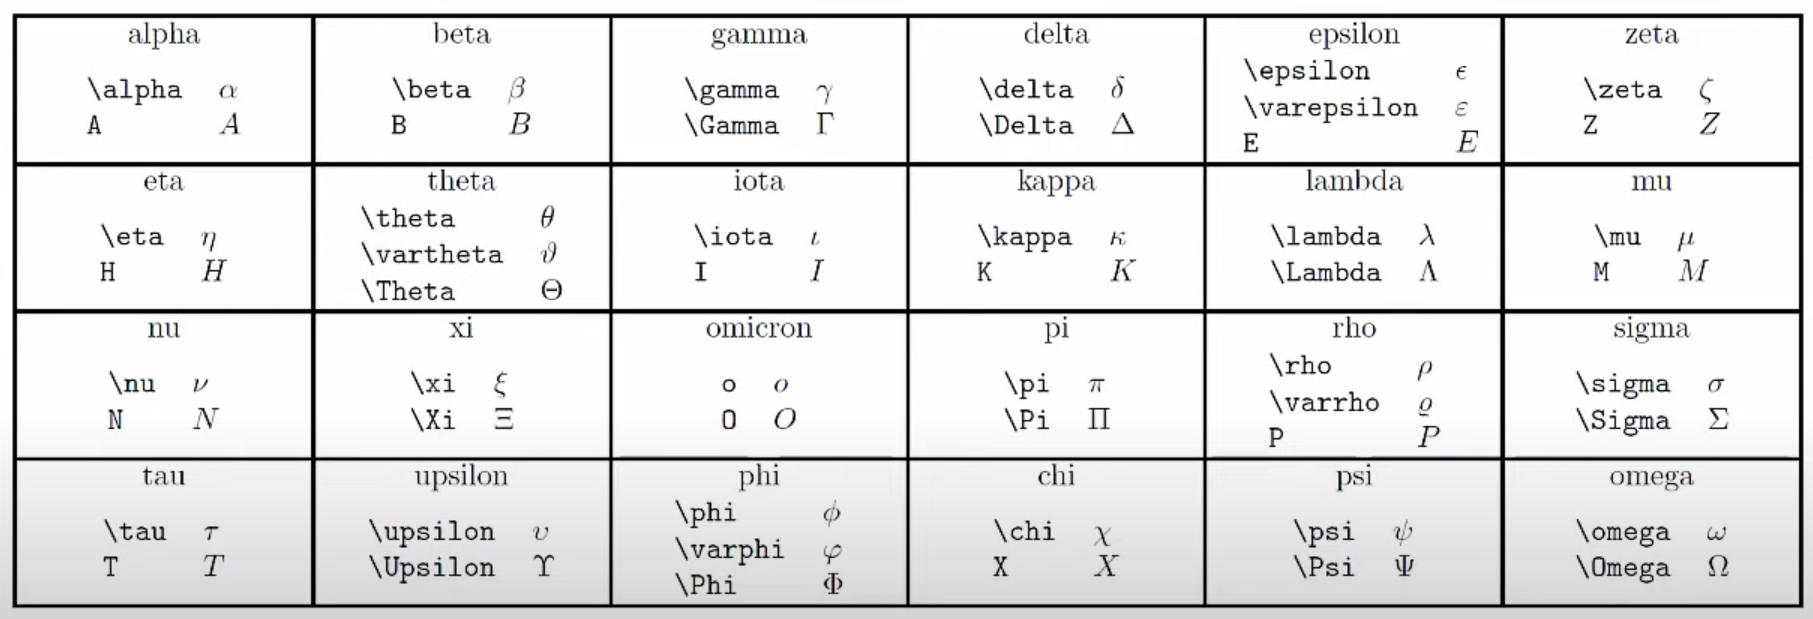
\includegraphics[width=\linewidth]{Greek_letters.png}

\subsection{Array}
\noindent \textbf{Warning: arrays must be generated in math mode}
\[
\begin{array}{ccc}
    \label{array: example}
    a_{11} & a_{12} & a_{13}  \\
    a_{21} & a_{22} & a_{23}  \\
    a_{31} & a_{32} & a_{33}
\end{array}
\]
The '\&' tells Latex where to align, while the slash tells where to start a new row.

\subsection{Calculus}
\begin{itemize}
    \item Limit
    \[
    \lim_{x \to \infty} \, \frac{1}{x}
    \]
    \item Sum
    \[
    \sum_{x=0}^{\infty} \, x^2
    \]
    \item Integral
    \[
    \int_{- \infty}^\infty x^2
    \]
    \begin{itemize}
        \item Double integral
        \[
        \iint_{- \infty}^\infty x^2
        \]
        \item Vertical bar for integral evaluation
        \[
        \int_0^4 x^2 \, = \frac{x^3}{3} \, \bigg\vert_0^4
        \]
    \end{itemize}
    \item Derivative
    \begin{itemize}
        \item Prime notation
        \[
        f'(x), f''(x), f'''(x), \ldots, f^{(n)}(x)
        \]
        \item Dot notation
        \[
        \dot{x}(t), \ddot{x}(t)
        \]
    \end{itemize}
    \item Vector
    \begin{itemize}
        \item Bold notation
        \[
        \bm{a}, \bm {b}, \bm{a} \cdot \bm {b}
        \]
        \item Arrow notation
        \[
        \vv{a}, \vv{b}, \vv{a} \times \vv{b}
        \]
    \end{itemize}
\end{itemize}
\subsection{Others}
\begin{itemize}
    \item Fraction
    \[
    \frac{3}{5}, \; \frac{x^2}{x+1}
    \]
    \item Square root
    \[ \sqrt{5} \]
    Can also specify the order:
    \[ \sqrt[3]{5} \]
    \item Comparison symbols
    Greater than or equal to: \( a \geq b\)
    
    Less than or equal to: \( a \leq b\)
    
    Approximately equal to: \(a \approx b\)
\end{itemize}

\section{Customization}
\subsection{Page breaks}
\begin{itemize}
    \item Soft break
    The 'pagebreak' command tries to extend the line spacing so that the text can occupy the whole page
    \item Hard break
    The 'newpage' command just starts a new page
\end{itemize}
\subsection{User defined commands}
\noindent \textbf{(Should be defined in preamble)} \\
First define a new command: I want the command 'veca' be the arrow-formed vector a.

Then try it out: \veca

\subsection{User defined functions}
\noindent \textbf{(Should be defined in preamble)}

\noindent I want to define 'myfunction' as a Fun. (It should be displayed without italics in math mode)

\noindent Try it out:

\[\MyFunction(x)\]

\subsection{Labels and references}
We have discussed how to change the text size in Section~\ref{sec: text size}, if you are unclear, please check them out.

The demonstration for generating an array is located in Section~\ref{array: example}, feel free to check them out.

\section{Ending remarks}
This is basically all for this tutorial, for more detailed information, please reference \href{https://www.youtube.com/watch?v=fCzF5gDy60g&list=WL&index=1}{this Youtube video}

\end{document}
